% Aberdeen style guide should be followed when using this
% layout. Their template powerpoint slide is used to extract the
% Aberdeen color and logo but is otherwise ignored (it has little or
% no formatting in it anyway).
%
% http://www.abdn.ac.uk/documents/style-guide.pdf

%%%%%%%%%%%%%%%%%%%% Document Class Settings %%%%%%%%%%%%%%%%%%%%%%%%%
% Pick if you want slides, or draft slides (no animations)
%%%%%%%%%%%%%%%%%%%%%%%%%%%%%%%%%%%%%%%%%%%%%%%%%%%%%%%%%%%%%%%%%%%%%%
%Normal document mode%
\documentclass[10pt,compress]{beamer}
%Draft or handout mode
%\documentclass[10pt,compress,handout]{beamer}
%\documentclass[10pt,compress,handout,ignorenonframetext]{beamer}

\renewcommand{\insertframenumber}{\theframenumber}
\renewcommand{\theframenumber}{\thesection-\arabic{framenumber}}
\renewcommand{\thesubsectionslide}{\thesection-\arabic{framenumber}}
\setbeamertemplate{headline}[text line]{This is frame: \insertframenumber}
\AtBeginSection{\setcounter{framenumber}{0}}

%%%%%%%%%%%%%%%%%%%% General Document settings %%%%%%%%%%%%%%%%%%%%%%%
% These settings must be set for each presentation
%%%%%%%%%%%%%%%%%%%%%%%%%%%%%%%%%%%%%%%%%%%%%%%%%%%%%%%%%%%%%%%%%%%%%%
\newcommand{\shortname}{jefferson.gomes@abdn.ac.uk} 
\newcommand{\fullname}{Dr Jeff Gomes}
\institute{School of Engineering}
\newcommand{\emailaddress}{}%jefferson.gomes@abdn.ac.uk}
\newcommand{\logoimage}{../FigBanner/UoAHorizBanner}
\title{Engineering Thermodynamics (EG3521)}
\subtitle{Module 2: Production of Power from Heat -- Gas Power Systems} 
\date[2014-15]{2014-15}

%%%%%%%%%%%%%%%%%%%% Template settings %%%%%%%%%%%%%%%%%%%%%%%%%%%%%%%
% You shouldn't have to change below this line, unless you want to.
%%%%%%%%%%%%%%%%%%%%%%%%%%%%%%%%%%%%%%%%%%%%%%%%%%%%%%%%%%%%%%%%%%%%%%
\usecolortheme{whale}
\useoutertheme{infolines}

% Use the fading effect for items that are covered on the current
% slide.
\beamertemplatetransparentcovered

% We abuse the author command to place all of the slide information on
% the title page.
\author[\shortname]{%
  \fullname\\\ttfamily{\emailaddress}
}


%At the start of every section, put a slide indicating the contents of the current section.
\AtBeginSection[] {
  \begin{frame}
    \frametitle{Section Outline}
    \tableofcontents[currentsection]
  \end{frame}
}

% Allow the inclusion of movies into the Presentation! At present,
% only the Okular program is capable of playing the movies *IN* the
% presentation.
\usepackage{multimedia}
\usepackage{animate}

%% Handsout -- comment out the lines below to create handstout with 4 slides in a page with space for comments
\usepackage{handoutWithNotes}

\mode<handout>
{
\usepackage{pgf,pgfpages}

\pgfpagesdeclarelayout{2 on 1 boxed with notes}
{
\edef\pgfpageoptionheight{\the\paperheight} 
\edef\pgfpageoptionwidth{\the\paperwidth}
\edef\pgfpageoptionborder{0pt}
}
{
\setkeys{pgfpagesuselayoutoption}{landscape}
\pgfpagesphysicalpageoptions
    {%
        logical pages=4,%
        physical height=\pgfpageoptionheight,%
        physical width=\pgfpageoptionwidth,%
        last logical shipout=2%
    } 
\pgfpageslogicalpageoptions{1}
    {%
    border code=\pgfsetlinewidth{1pt}\pgfstroke,%
    scale=1,
    center=\pgfpoint{.25\pgfphysicalwidth}{.75\pgfphysicalheight}%
    }%
\pgfpageslogicalpageoptions{2}
    {%
    border code=\pgfsetlinewidth{1pt}\pgfstroke,%
    scale=1,
    center=\pgfpoint{.25\pgfphysicalwidth}{.25\pgfphysicalheight}%
    }%
\pgfpageslogicalpageoptions{3}
    {%
    border shrink=\pgfpageoptionborder,%
    resized width=.7\pgfphysicalwidth,%
    resized height=.5\pgfphysicalheight,%
    center=\pgfpoint{.75\pgfphysicalwidth}{.29\pgfphysicalheight},%
    copy from=3
    }%
\pgfpageslogicalpageoptions{4}
    {%
    border shrink=\pgfpageoptionborder,%
    resized width=.7\pgfphysicalwidth,%
    resized height=.5\pgfphysicalheight,%
    center=\pgfpoint{.75\pgfphysicalwidth}{.79\pgfphysicalheight},%
    copy from=4
    }%

\AtBeginDocument
    {
    \newbox\notesbox
    \setbox\notesbox=\vbox
        {
            \hsize=\paperwidth
            \vskip-1in\hskip-1in\vbox
            {
                \vskip1cm
                Notes\vskip1cm
                        \hrule width\paperwidth\vskip1cm
                    \hrule width\paperwidth\vskip1cm
                        \hrule width\paperwidth\vskip1cm
                    \hrule width\paperwidth\vskip1cm
                        \hrule width\paperwidth\vskip1cm
                    \hrule width\paperwidth\vskip1cm
                    \hrule width\paperwidth\vskip1cm
                    \hrule width\paperwidth\vskip1cm
                        \hrule width\paperwidth
            }
        }
        \pgfpagesshipoutlogicalpage{3}\copy\notesbox
        \pgfpagesshipoutlogicalpage{4}\copy\notesbox
    }
}
}

%\pgfpagesuselayout{2 on 1 boxed with notes}[letterpaper,border shrink=5mm]
%\pgfpagesuselayout{2 on 1 boxed with notes}[letterpaper,border shrink=5mm]

%%%%% Color settings
\usepackage{color}
%% The background color for code listings (i.e. example programs)
\definecolor{lbcolor}{rgb}{0.9,0.9,0.9}%
\definecolor{UoARed}{rgb}{0.64706, 0.0, 0.12941}
\definecolor{UoALight}{rgb}{0.85, 0.85, 0.85}
\definecolor{UoALighter}{rgb}{0.92, 0.92, 0.92}
\setbeamercolor{structure}{fg=UoARed} % General background and higlight color
\setbeamercolor{frametitle}{bg=black} % General color
\setbeamercolor{frametitle right}{bg=black} % General color
\setbeamercolor{block body}{bg=UoALighter} % For blocks
\setbeamercolor{structure}{bg=UoALight} % For blocks
% Rounded boxes for blocks
\setbeamertemplate{blocks}[rounded]

%%%%% Font settings
% Aberdeen requires the use of Arial in slides. We can use the
% Helvetica font as its widely available like so
% \usepackage{helvet}
% \renewcommand{\familydefault}{\sfdefault}
% But beamer already uses a sans font, so we will stick with that.

% The size of the font used for the code listings.
\newcommand{\goodsize}{\fontsize{6}{7}\selectfont}

% Extra math packages, symbols and colors. If you're using Latex you
% must be using it for formatting the math!
\usepackage{amscd,amssymb} \usepackage{amsfonts}
\usepackage[mathscr]{eucal} \usepackage{mathrsfs}
\usepackage{latexsym} \usepackage{amsmath} \usepackage{bm}
\usepackage{amsthm} \usepackage{textcomp} \usepackage{eurosym}
% This package provides \cancel{a} and \cancelto{a}{b} to "cancel"
% expressions in math.
\usepackage{cancel}

\usepackage{comment} 

% Get rid of font warnings as modern LaTaX installations have scalable
% fonts
\usepackage{type1cm} 

%\usepackage{enumitem} % continuous numbering throughout enumerate commands

% For exact placement of images/text on the cover page
\usepackage[absolute]{textpos}
\setlength{\TPHorizModule}{1mm}%sets the textpos unit
\setlength{\TPVertModule}{\TPHorizModule} 

% Source code formatting package
\usepackage{listings}%
\lstset{ backgroundcolor=\color{lbcolor}, tabsize=4,
  numberstyle=\tiny, rulecolor=, language=C++, basicstyle=\goodsize,
  upquote=true, aboveskip={1.5\baselineskip}, columns=fixed,
  showstringspaces=false, extendedchars=true, breaklines=false,
  prebreak = \raisebox{0ex}[0ex][0ex]{\ensuremath{\hookleftarrow}},
  frame=single, showtabs=false, showspaces=false,
  showstringspaces=false, identifierstyle=\ttfamily,
  keywordstyle=\color[rgb]{0,0,1},
  commentstyle=\color[rgb]{0.133,0.545,0.133},
  stringstyle=\color[rgb]{0.627,0.126,0.941}}

% Allows the inclusion of other PDF's into the final PDF. Great for
% attaching tutorial sheets etc.
\usepackage{pdfpages}
\setbeamercolor{background canvas}{bg=}  

% Remove foot note horizontal rules, they occupy too much space on the slide
\renewcommand{\footnoterule}{}

% Force the driver to fix the colors on PDF's which include mixed
% colorspaces and transparency.
\pdfpageattr {/Group << /S /Transparency /I true /CS /DeviceRGB>>}

% Include a graphics, reserve space for it but
% show it on the next frame.
% Parameters:
% #1 Which slide you want it on
% #2 Previous slides
% #3 Options to \includegraphics (optional)
% #4 Name of graphic
\newcommand{\reserveandshow}[4]{%
\phantom{\includegraphics<#2|handout:0>[#3]{#4}}%
\includegraphics<#1>[#3]{#4}%
}

\newcommand{\frc}{\displaystyle\frac}
\newcommand{\red}{\textcolor{red}}
\newcommand{\blue}{\textcolor{blue}}
\newcommand{\green}{\textcolor{green}}
\newcommand{\purple}{\textcolor{purple}}
 

\begin{document}

% Title page layout
\begin{frame}
  \titlepage
  \vfill%
  \begin{center}
    \includegraphics[clip,width=0.8\textwidth]{\logoimage}
  \end{center}
\end{frame}

% Table of contents
%\frame{ \frametitle{Slides Outline}
%  \tableofcontents
%}


%%%%%%%%%%%%%%%%%%%% The Presentation Proper %%%%%%%%%%%%%%%%%%%%%%%%%
% Fill below this line with \begin{frame} commands! It's best to
% always add the fragile option incase you're going to use the
% verbatim environment.
%%%%%%%%%%%%%%%%%%%%%%%%%%%%%%%%%%%%%%%%%%%%%%%%%%%%%%%%%%%%%%%%%%%%%%

%%%
%%% SECTION
%%%
\section{Introduction}

%%%===            ===%%%
%%%=== SUBSECTION ===%%%
%%%===            ===%%%
\subsection{Motivation}
%%%
%%% Slide
%%%
\begin{frame}
 \frametitle{Aims and Objectives}
 At the end of this set of lectures, you should be able to:
 \begin{enumerate}[(i)]
  \item <1-> Assess the performance of \red{gas power cycles};
  \item <2-> Solve problems based on the Brayton, Otto and Diesel cycles;
  \item <3-> Perform second-law analysis of gas power cycles and;
  \item <4-> Solve problems based on the Brayton cycle;
  \item <5-> Identify simplifying assumptions for second-law analysis of gas power cycles.
 \end{enumerate}
\end{frame}


%%%===            ===%%%
%%%=== SUBSECTION ===%%%
%%%===            ===%%%
\subsection{Bibliography} 
%%%
%%% Slide
%%%
\begin{frame}
 \frametitle{Suggested References}
  \begin{enumerate}[1]\scriptsize
   \item M.J. Moran, H.N. Saphiro, D.D. Boettner, M.B. Bailey, $\lq$Principles of Engineering Thermodynamics',  7$^{th}$ Edition: Chapter 9;
   \item J.M. Smith, H.C. Van Ness, M.M. Abbott, $\lq$Introduction to Chemical Engineering Thermodynamics', 6$^{th}$ Edition: Chapter 8;
   %\item A.B. Pippard, $\lq$Elements of Classical Thermodynamics' (1966): Chapters 2, 3 and 4;
   \item I. Muller, W.H. Muller, $\lq$Fundamentals of Thermodynamics and Applications', Chapter 3;
   \item C. Borgnakke, R.E. Sonntag, $\lq$Fundamentals of Thermodynamics -- SI Version', 8$^{th}$ Edition: Chapter 10;
   \item \href{http://www.learnthermo.com}{http://www.learnthermo.com}, Chapter 9.
   \item S.-S. Hou (2007) $\lq$Comparison of Performances of Air-Standard Atkinson and Otto Cycles with Heat Transfer Considerations', \href{http://dx.doi.org/10.1016/j.enconman.2006.11.001}{{\it Energy Conversion and Management} 48:1683-1690}.
   \item Y. Ge {\it et al.} (2006) $\lq$Performance of an Atkinson Cycle with Heat Transfer, Friction and Variable Specific-Heats of the Working Fluid', \href{http://dx.doi.org/10.1016/j.apenergy.2005.12.003}{{\it Applied Energy} 83:1210-1221}.
   \item P. Spittle (2003) \href{http://dx.doi.org/10.1088/0031-9120/38/6/002}{$\lq$Gas Turbine Technology'}, {\it Physics Education}, 38:504-511.
  \end{enumerate}
\end{frame}


%%%===            ===%%%
%%%=== SUBSECTION ===%%%
%%%===            ===%%%
\subsection{Initial Assumptions}
%%%
%%% Slide
%%%
\begin{frame}
 \frametitle{Air Standard Efficiency}
   \begin{columns}
     \begin{column}[c]{0.5\linewidth}
       \begin{enumerate} \scriptsize
         \item<1-> In the first part of this Module we revised the definition of \textcolor{blue}{cycles} in which fuel is $\lq$burned' in a \textcolor{blue}{combustion chamber} with air, resulting in a stream of combustion products, i.e.;
         \item<2-> Due to the complexity on thermodynamics analysis of gas power cycle, we will assume that \textcolor{blue}{air is the only work fluid} with an external heat source;
         \item<3-> Air behaves as an ideal gas with contant heat capacities at room temperature $\left(\text{MW = 29 g.mol}^{-1},\text{ C}_{p}\text{ = 1.005 kJ.(kg.K)}^{-1}\right.$ and C$\left._{v}\text{ = 0.718 kJ.(kg.K)}^{-1}\right)$;
         \item<4-> Compression and expansion processes are adiabatic and with no internal friction;
         \item<5-> Exhausted process is replaced by a heat-rejection process that restores the working fluid to its initial state;
         \item<6-> Cycles in which the above is applied are called \textcolor{blue}{Air-Standard Cycles};
         \item<7-> The efficiency of an engine using air as the working medium is called \textcolor{blue}{air standard efficiency} or \textcolor{blue}{ideal efficiency};
       \end{enumerate}
     \end{column}  
     \begin{column}[c]{0.5\linewidth}
       \visible<1->{\begin{figure}%
         \begin{center}
           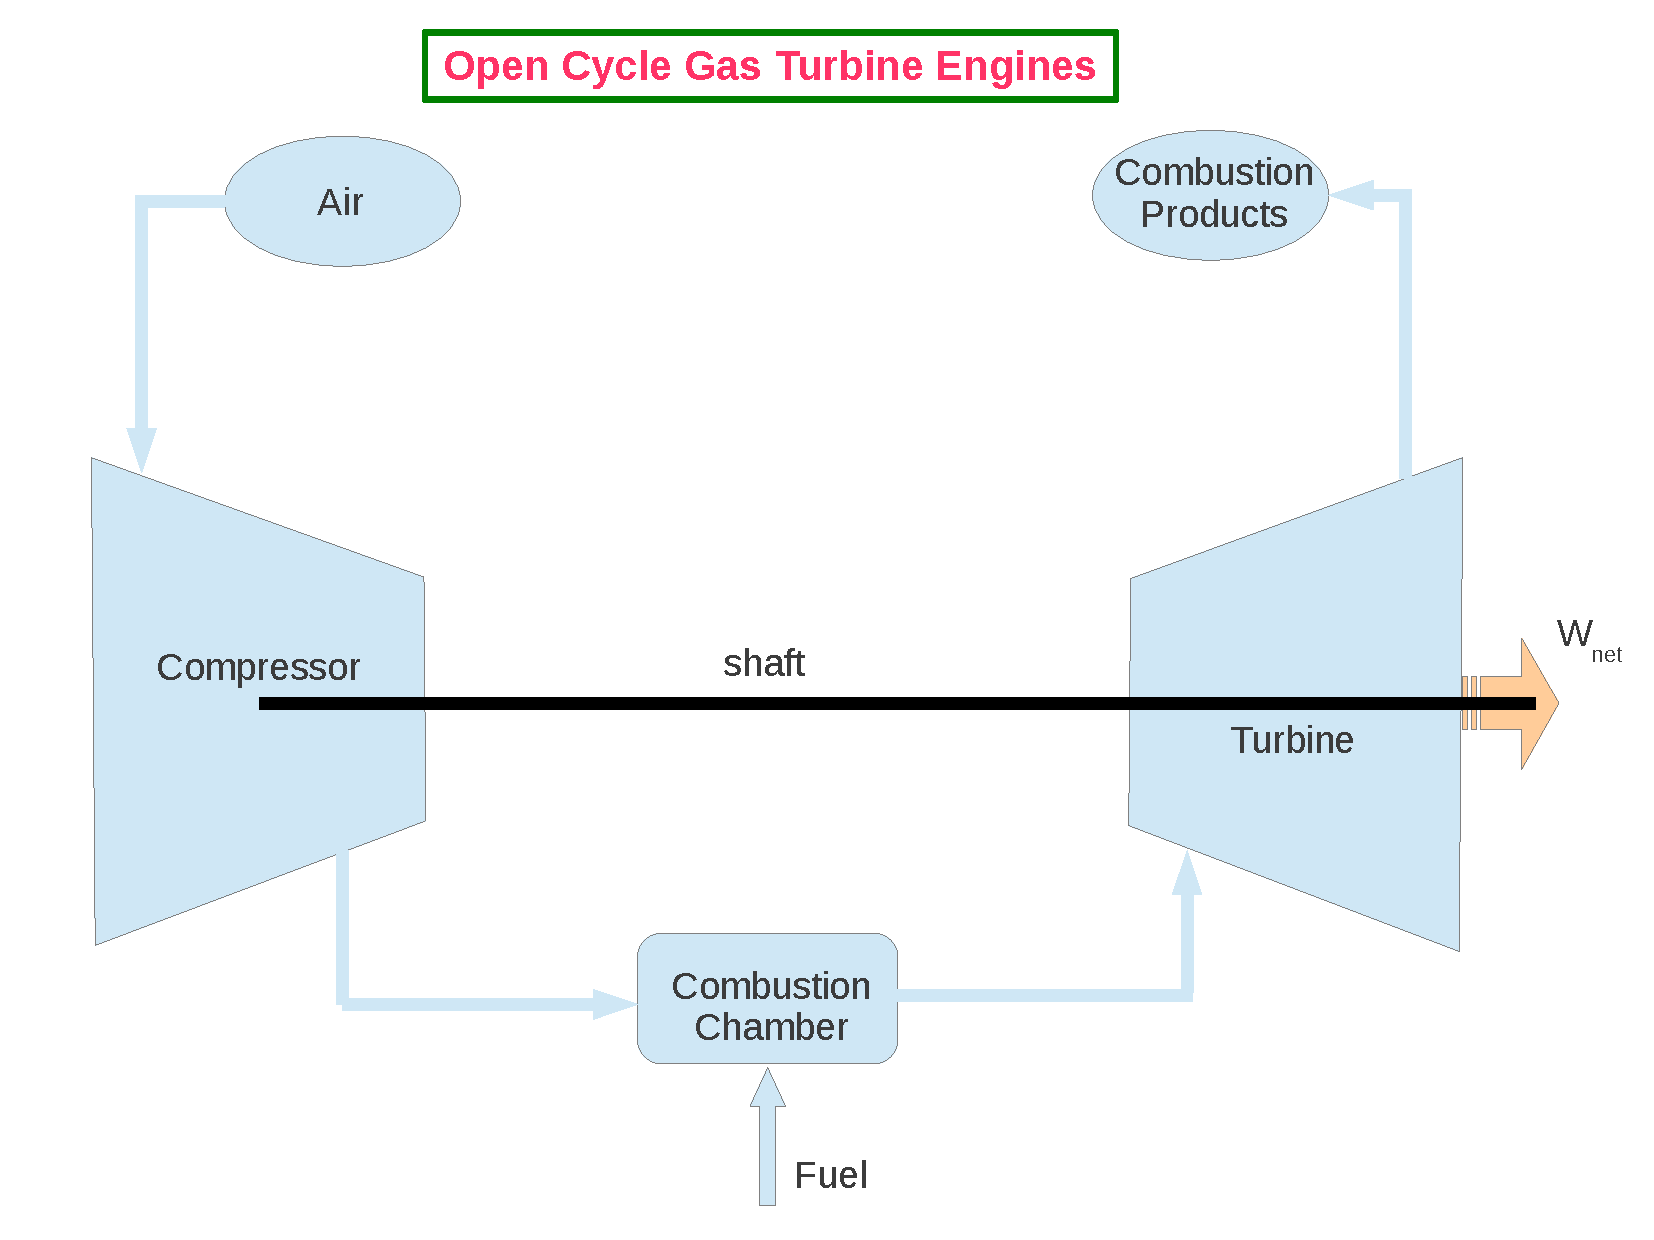
\includegraphics[width=5.8cm,clip]{./Pics/Open_Gas_Turbine_Engines}
         \end{center}
       \end{figure}} 
       \begin{enumerate}\setcounter{enumi}{7} \scriptsize
          \item<8-> In order to compare ideal and actual/real efficiencies, we introduce the relative efficiency:
             \visible<8->{\begin{equation}
                \textcolor{blue}{\eta_{\text{relative}}=\displaystyle\frac{\text{Actual Thermal Efficiency}}{\text{Air-Standard Efficiency}}}
             \end{equation}}
       \end{enumerate}
     \end{column}   
  \end{columns}  
\end{frame}


%%%
%%% SECTION
%%%
\section{Internal Combustion Engines}

%%%===            ===%%%
%%%=== SUBSECTION ===%%%
%%%===            ===%%%
\subsection{Reciprocating Engines}

%%%
%%% Slide
%%%
\begin{frame}
 \frametitle{Nomenclature}
 \begin{columns}
  \begin{column}[c]{0.5\linewidth}
   \begin{enumerate}[(1)]\scriptsize
    \item<1-> Components:
      \begin{enumerate}[(a)]\scriptsize
        \item<1-> \blue{Bottom Dead Center (BDC)}: position of the piston in which the volume becomes \red{maximum};
        \item<1-> \blue{Top Dead Center (TDC)}: position of the piston in which the volume becomes \red{minimum} (i.e., \underline{clearance volume});
        \item<1-> \blue{Bore}: diameter of the piston;
        \item<1-> The \blue{Intake Valve} is responsible to control the inflow of the air-fuel solution into the cylinder;
        \item<1-> The \blue{Exhaust Valve} lets the combustion gases leave the cylinder;
      \end{enumerate} 
    \item<2-> \blue{Stroke}: the largest distance that the piston can travel: $X_{\text{TDC}}-X_{\text{BDC}}$;
    \item<2-> \blue{Displacement Volume}: volume of the cylinder limited by $X_{\text{TDC}}$ and $X_{\text{BDC}}$
    \item<3-> \blue{Compression Ratio}: 
        \begin{equation}
           r = \frc{V_{\text{max}}}{V_{\text{min}}} = \frc{V_{\text{BDC}}}{V_{\text{TDC}}}
        \end{equation}
   \end{enumerate}
  \end{column}
  \begin{column}[c]{0.5\linewidth}
   \begin{figure}%
    \begin{center}
     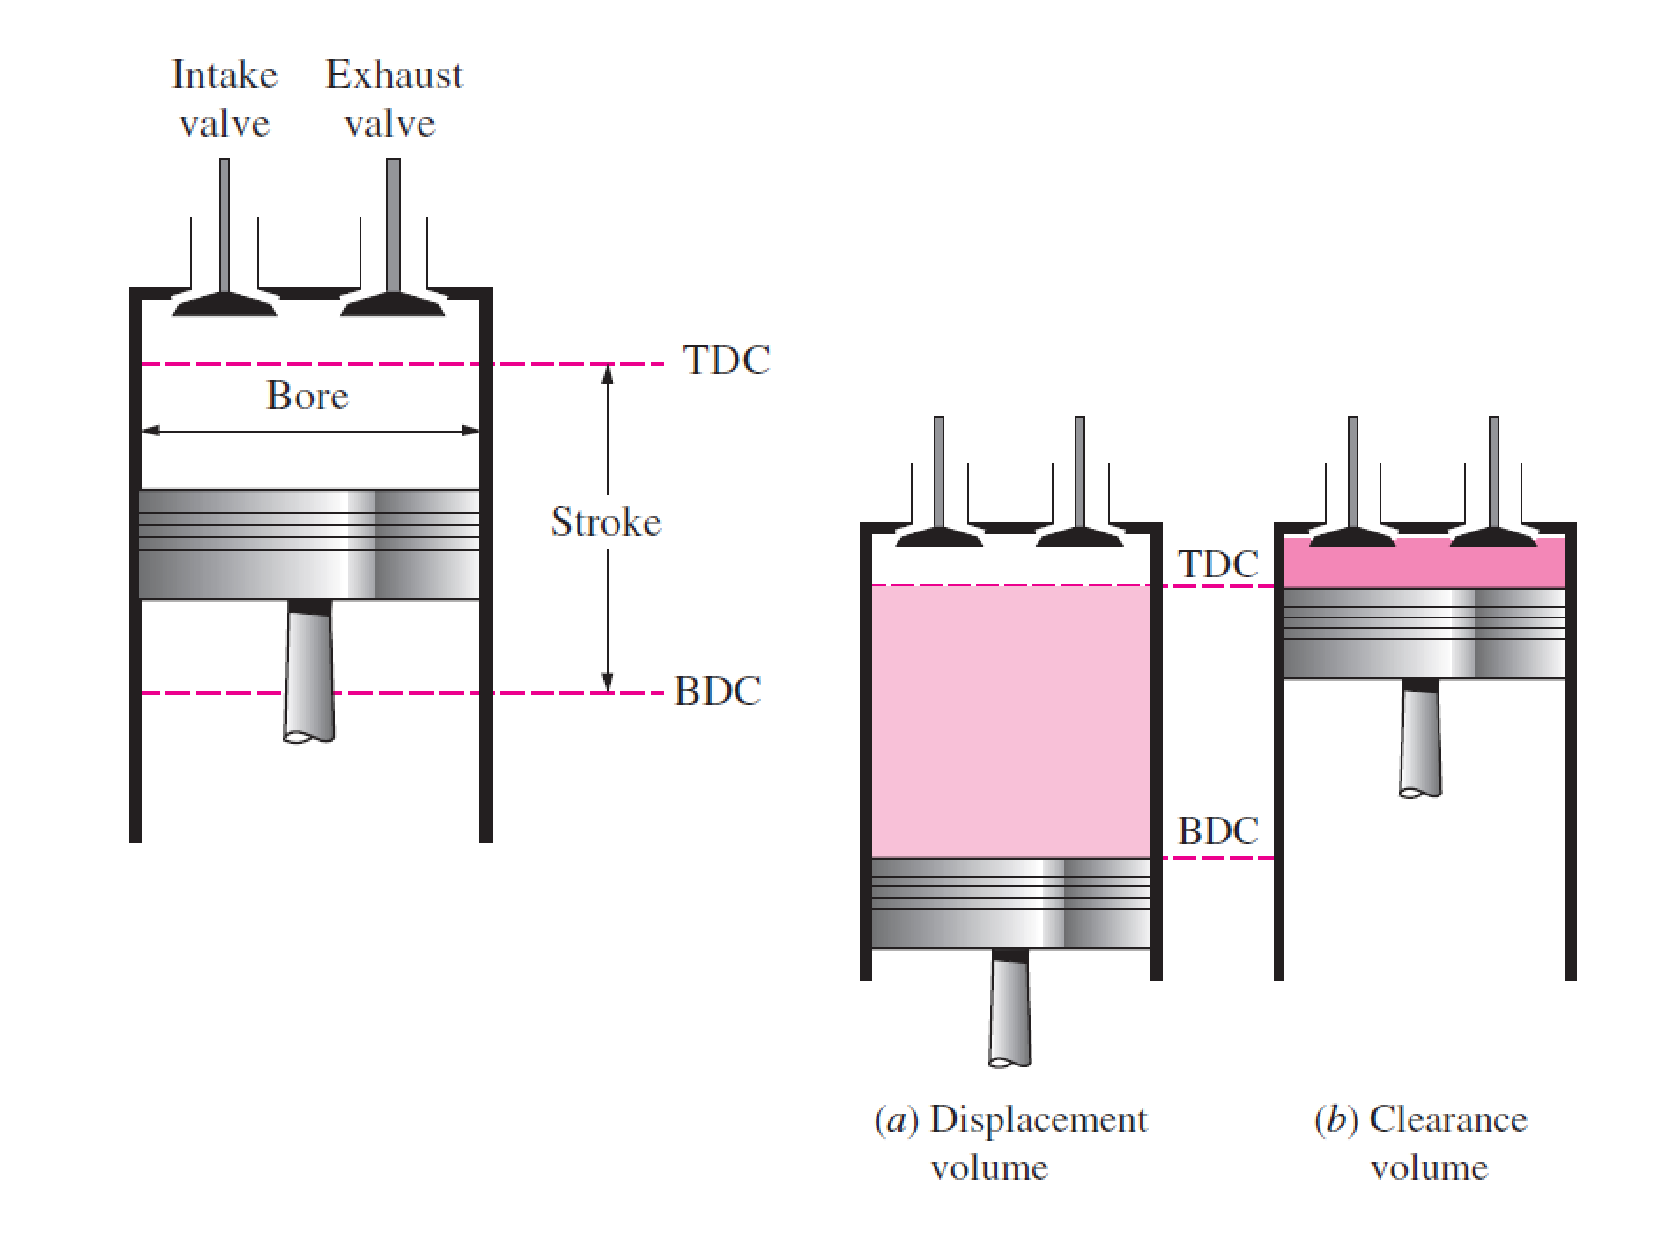
\includegraphics[width=6.2cm,clip]{./Pics/GasCycle_ReciprocatingEngine}
    \end{center}
   \end{figure} 
  \end{column}  
 \end{columns}
\end{frame}

%%%
%%% Slide
%%%
\begin{frame}
 \frametitle{Nomenclature}
 \begin{columns}
  \begin{column}[c]{0.5\linewidth}
   \begin{enumerate}[(1)]\setcounter{enumi}{4} \scriptsize
     \item<1-> The \blue{Mean Effective Pressure (MEP)} of the cycle is a fictitious pressure that, if it acted on the piston during the entire power stroke, would {\it produce the same amount of net work as that produced during the actual cycle}:
        \visible<1->{\begin{eqnarray}
          && W_{\text{net}} = MEP \times \text{Piston area} \times \text{Stroke} \nonumber \\
          && MEP= \frc{W_{\text{net}}}{V_{\text{max}}-V_{\text{min}}}
        \end{eqnarray}} 
     \item<2-> MEP is used as a parameter to compare performances of reciprocating engines of equal size:  \blue{Larger MEP $\Longrightarrow$ larger $W_{\text{net}}$}. 
   \end{enumerate}
  \end{column}
  \begin{column}[c]{0.5\linewidth}
   \begin{figure}%
    \begin{center}
     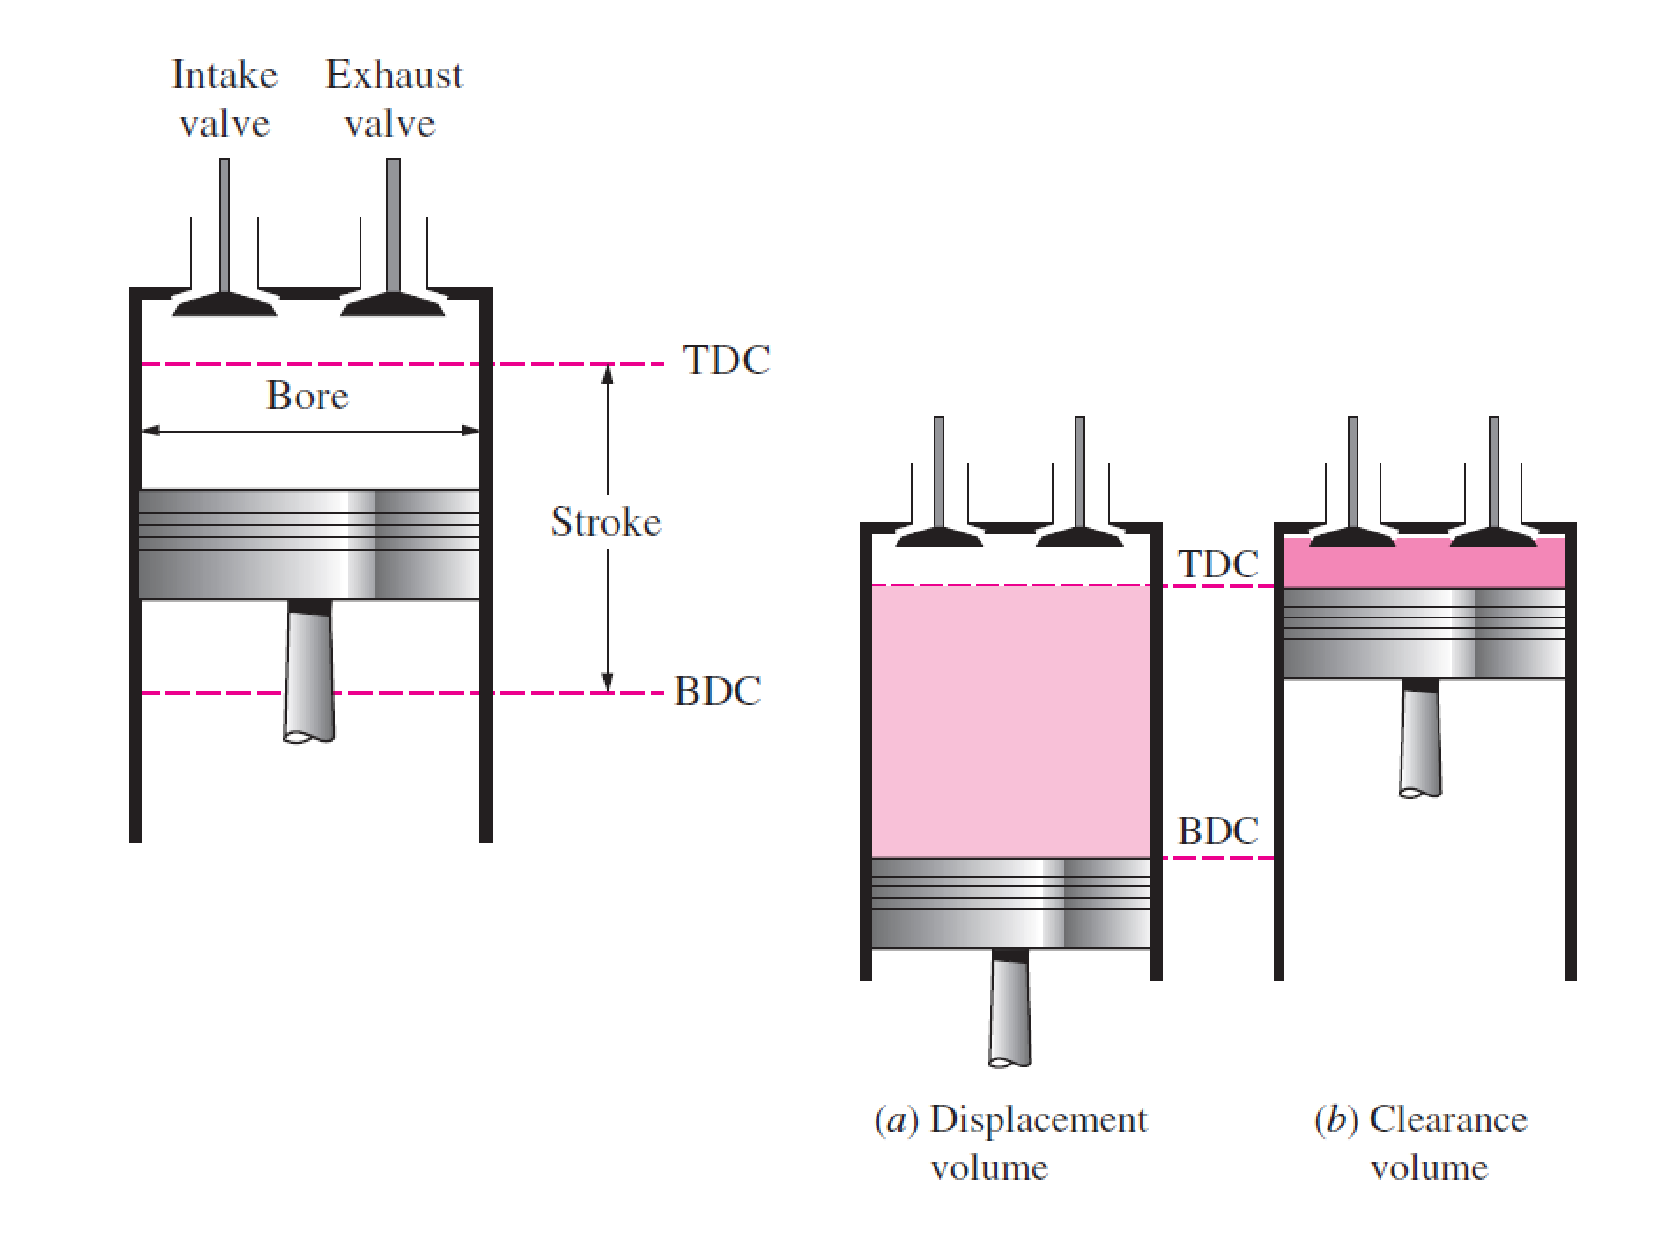
\includegraphics[width=6.2cm,clip]{./Pics/GasCycle_ReciprocatingEngine}
    \end{center}
   \end{figure} 
  \end{column}  
 \end{columns}
\end{frame}

%%%
%%% Slide
%%%
\begin{frame}
 \frametitle{Classification of Reciprocating Engines}
  \begin{columns}
   \begin{column}[c]{0.45\linewidth}\scriptsize
   
     \begin{enumerate}\scriptsize
      \item <2-> \blue{Spark Ignition (SI) Engines}: the combustion of the air–-fuel mixture is initiated by a spark plug (the mixture is at  \red{flash point} conditions);
       \begin{enumerate}\scriptsize
        %\item <4-> Fuel--air solution is compressed to $T<T_{\text{autoignition}}^{\text{fuel}}$ and combustion is initialised by a (electric) spark;
        \item <4-> Four stroke cycle: suction, compression, expansion (also called power or working) and exhaust;
        \item <5-> Two stroke cycle: compression and expansion;
       \end{enumerate}
      \item <3-> \blue{Compression Ignition (CI) Engines}: the air–-fuel mixture is self-ignited as a result of compressing the mixture above its self-ignition temperature.
       \begin{enumerate}\scriptsize
          \item <6-> \underline{Diesel cycle} is the ideal cycle for CI reciprocating engines;
          \item <7-> Strokes of the cycle: suction, compression, expansion and exhaust.
       \end{enumerate}
     \end{enumerate}
   \end{column}
   \begin{column}[c]{0.55\linewidth}
    \begin{figure}%
     \begin{center}
      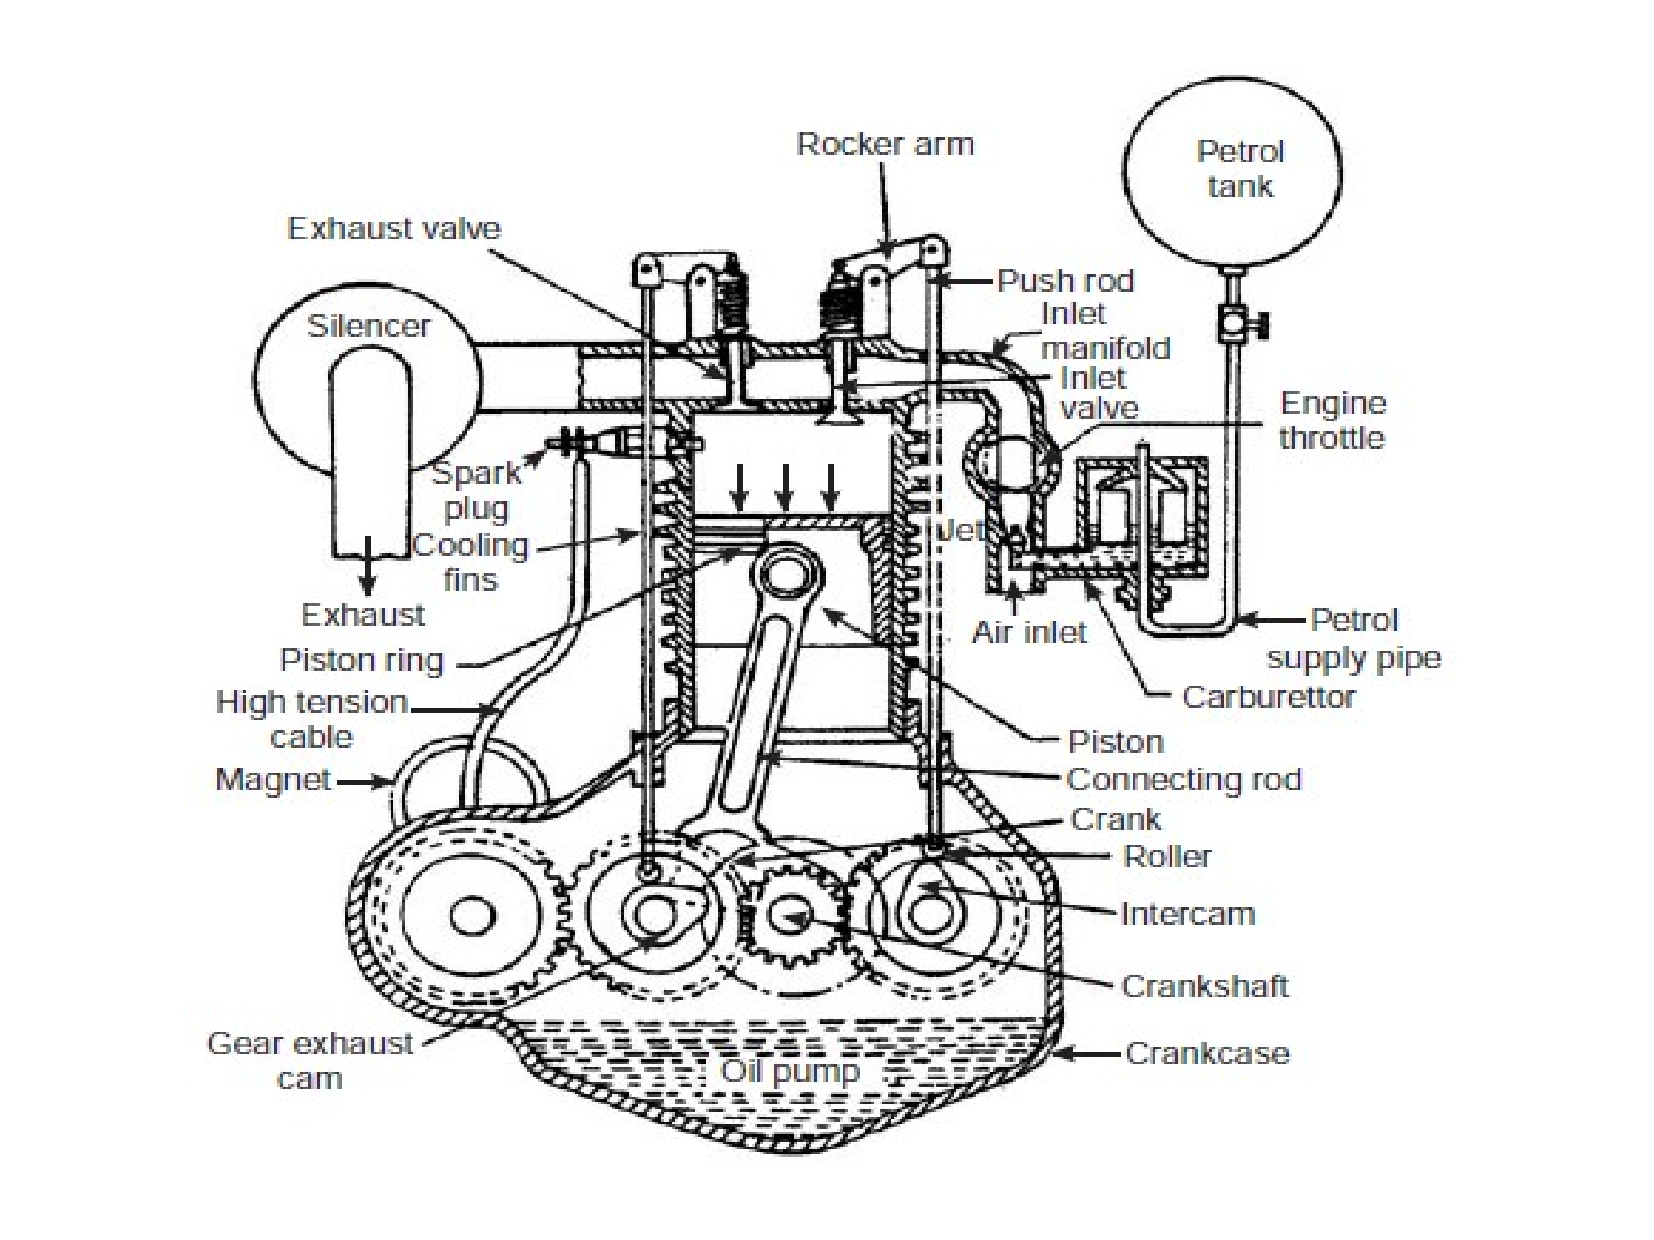
\includegraphics[width=7.5cm,clip]{./Pics/InternalCombustion_4Strokes}
      \scriptsize\caption{\scriptsize Air-cooled four-stroke petrol engine.}
     \end{center}
    \end{figure}  
   \end{column}  
  \end{columns}
\end{frame}


%%%===            ===%%%
%%%=== SUBSECTION ===%%%
%%%===            ===%%%
\subsection{Ideal Carnot Cycle}
%%%
%%% Slide
%%%
\begin{frame}
 \frametitle{Carnot Cycle}
 \begin{columns}
  \begin{column}[c]{0.45\linewidth}
   \begin{enumerate}[(1)] \scriptsize
     \item<1-> \blue{Carnot cycle} has the highest possible efficiency and, similarly from previous lectures, consists of four stages:
     \begin{itemize}\scriptsize
       \item<1-> {\bf 1-2}: Isothermal expansion; 
       \item<1-> {\bf 2-3}: Adiabatic expansion;
       \item<1-> {\bf 3-4}: Isothermal compression;
       \item<1-> {\bf 4-1}: Adiabatic compression.
     \end{itemize}\scriptsize
     \item <2-> The efficiency of the cycle is then given by
       \begin{eqnarray}
        \textcolor{blue}{\eta_{\text{Carnot}}} &=& \displaystyle\frac{\text{work done}}{\text{heat supplied}} \nonumber\\
                         &=& \displaystyle\frac{\text{heat supplied}-\text{heat rejected}}{\text{heat supplied}} \nonumber \\
                         &=& \displaystyle\frac{Q_{s}-Q_{r}}{Q_{s}} = \displaystyle\frac{T_{1}-T_{2}}{T_{1}} \nonumber  \\
                         &=&  \blue{1 - \frc{T_{2}}{T_{1}}}
       \end{eqnarray}
     \item<3-> The efficiency of the cycle can be readily enhanced if the $T_{2}$ decreases. And in the limit,
        \begin{displaymath}
           \lim_{T_{2} \to 0}\eta_{\text{Carnot}} = 1
        \end{displaymath}
   \end{enumerate}
  \end{column}
  \begin{column}[c]{0.55\linewidth}
   \begin{enumerate}[(1)]\setcounter{enumi}{3} \scriptsize
     \item<4-> We can not produce a system that can move
     \begin{enumerate}[(a)] \scriptsize
        \item<4-> very slow in the \blue{isothermal expansion} ($\lq$forward stroke') and;
        \item<4-> very fast during the remainder of the adiabatic expansion. 
     \end{enumerate}
     \item<5-> The cycle would become \red{unfeasible}.
   \end{enumerate} 
   \begin{figure}%
    \begin{center}
     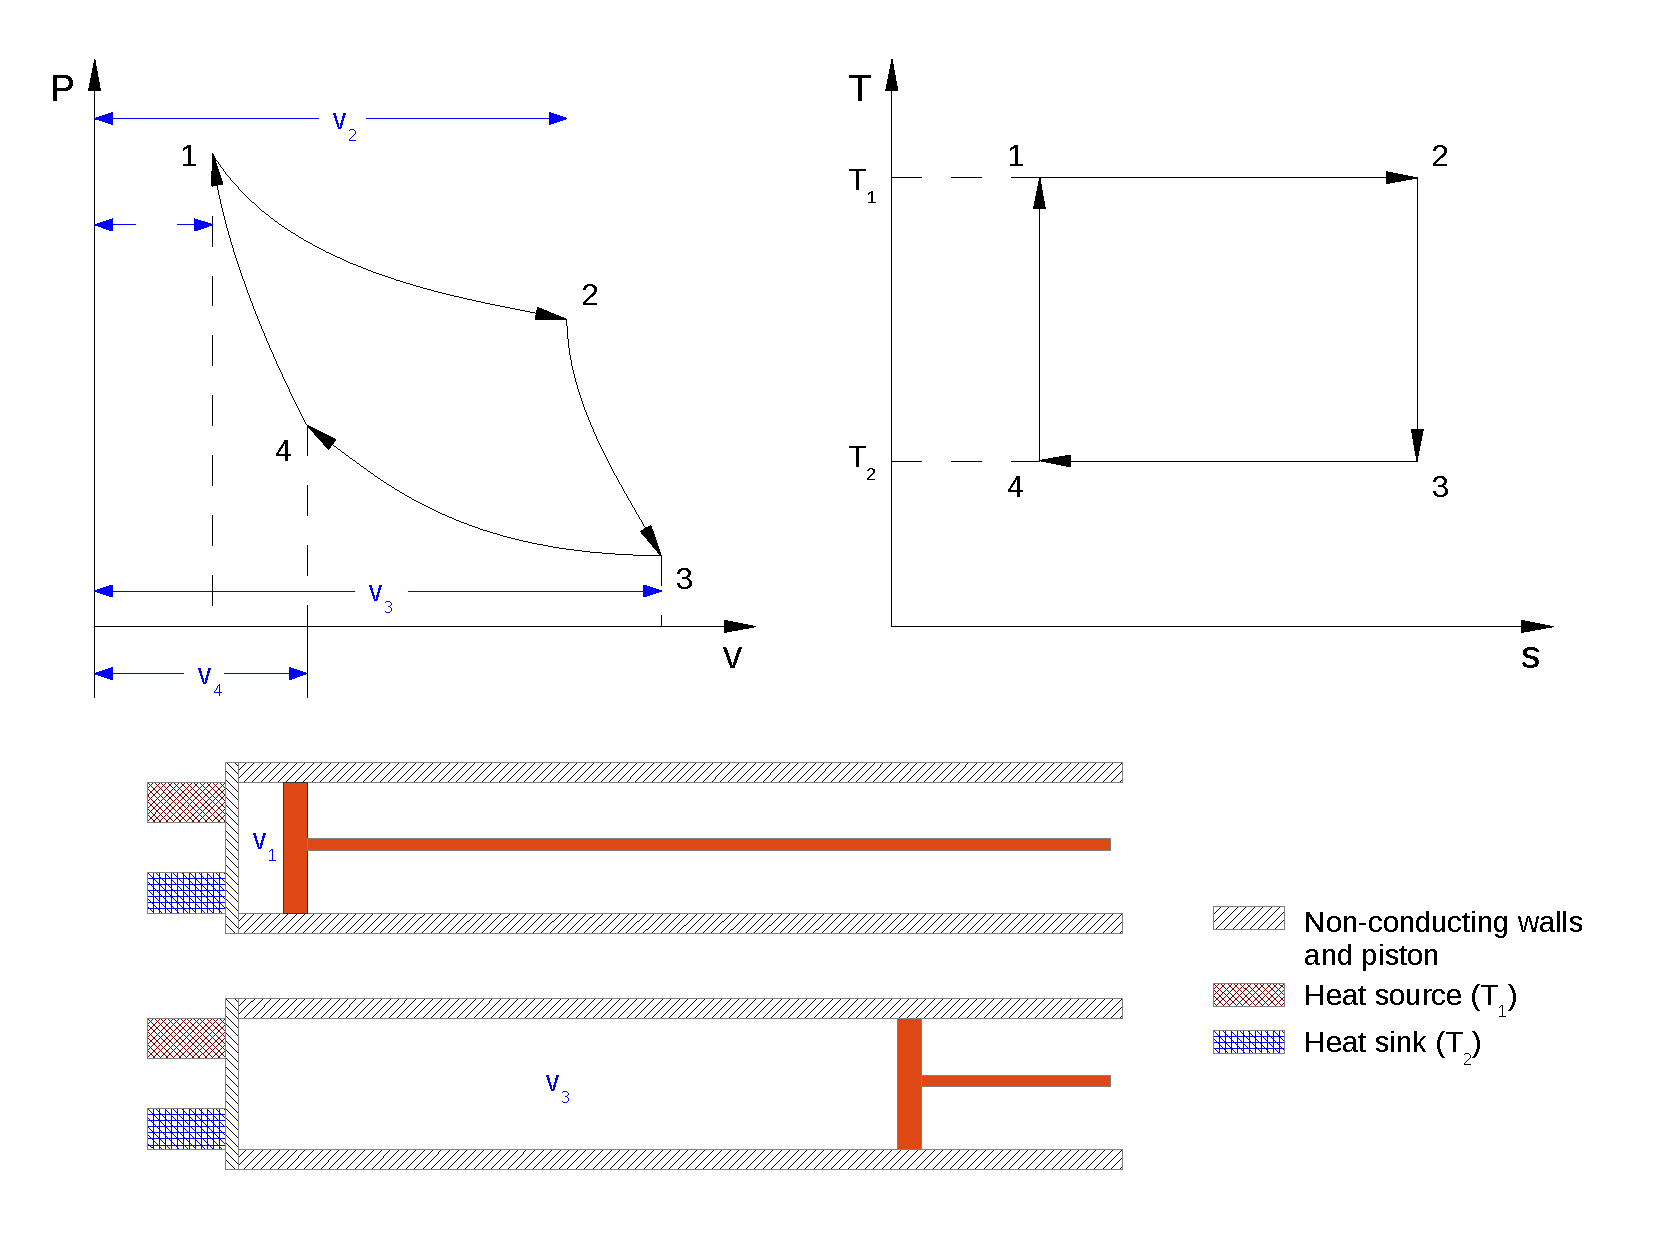
\includegraphics[width=6.5cm,clip]{./Pics/Carnot_Reciprocating}
    \end{center}
   \end{figure} 
  \end{column}  
 \end{columns} 
\end{frame}

%%%
%%% Slide
%%%
\begin{frame}
 \frametitle{Carnot Cycle -- Example}
     In a Carnot cycle, the maximum pressure and temperature are limited to 18 bar and 410$^{\circ}$C. The ratio of isentropic compression and isothermal expansion are 6 and 1.5, respectively. Assuming the volume of the air at the beginning of isothermal expansion is 0.18 m$^{3}$, determine:
       \begin{enumerate}[(a)]
          \item Temperature and pressures at all stages of the cycle; 
          \item Change in entropy during isothermal expansion; 
          \item Mean thermal efficiency of the cycle; 
          \item Mean effective pressure (MEP) of the cycle and;
          \item Theoretical power if there are 210 working cycles per minute.
       \end{enumerate}
\end{frame}



%%%===            ===%%%
%%%=== SUBSECTION ===%%%
%%%===            ===%%%
\subsection{Otto Cycle (Constant Volume)}

%%%
%%% Slide
%%%
\begin{frame}
 \frametitle{Four-Strokes Internal Combustion Engines}
  \begin{columns}
   \begin{column}[c]{0.4\linewidth}
    \begin{enumerate}[(1)]\scriptsize
     \item<1-> Fuel--air solution is compressed to a \blue{temperature just below the auto--ignition temperature of the fuel} and combustion is initialised by an electric spark;
     \item<2-> \blue{Suction stroke (SS):} also called \blue{intake stroke}. The mixture is injected through the intake valve (IV). The exhaust valve (EV) remains closed during this stage;
     \item<3-> \red{Compression stroke (CS):} whereas IV and EV remain closed, pressure and temperature of the solution rise. Near the end of CS, the fuel is ignited by an electric spark, leading to the combustion of the fuel (consumption of carbon);
     \item<4-> \blue{Expansion stroke (WS):} also called \blue{power} or \blue{working} stroke. IV and EV remain closed and near the completion of the this stroke, the \blue{EV} is opened and the pressure in the cylinder push most of the gases out of the cylinder;
    \end{enumerate}
   \end{column}
   \begin{column}[c]{0.6\linewidth}
    \begin{figure}%
     \begin{center}
      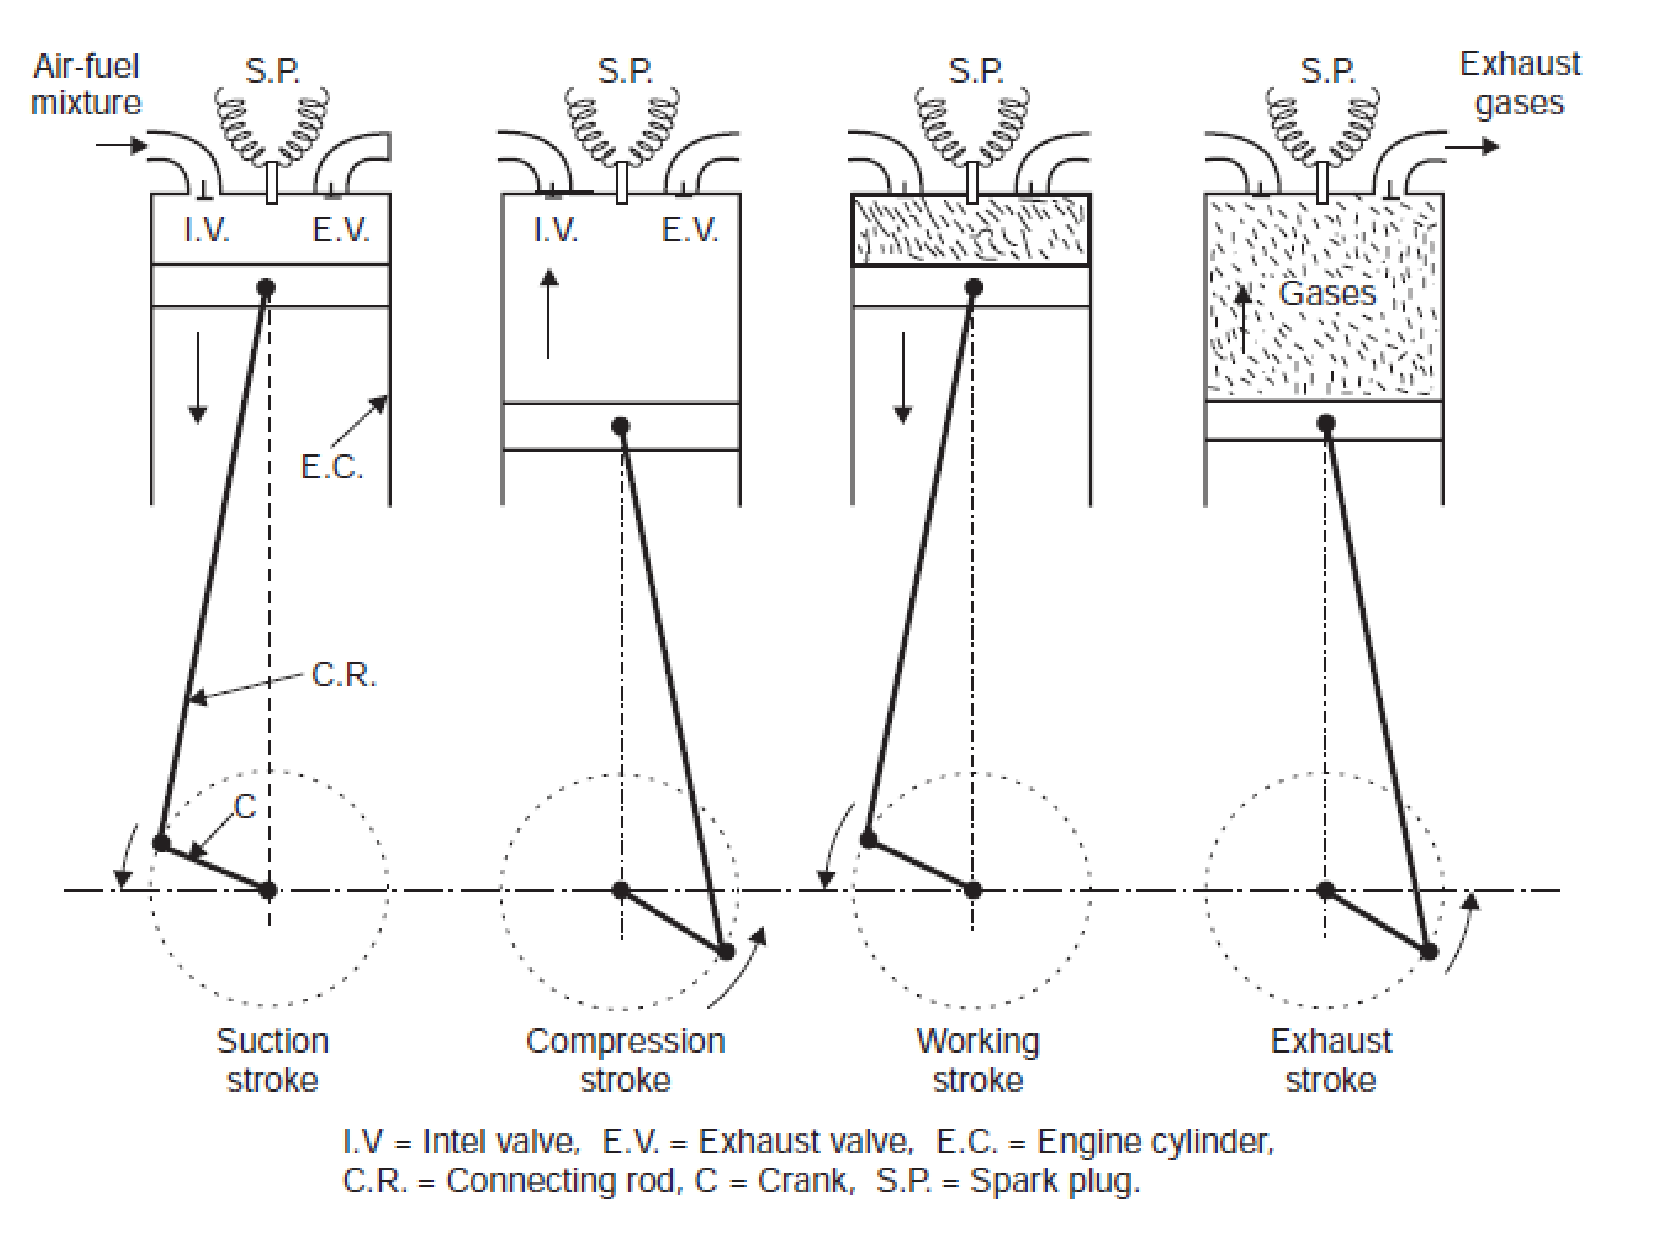
\includegraphics[width=6.5cm,clip]{./Pics/InternalCombustion_4Strokes_Otto}
      %\caption{Air-cooled four-stroke petrol engine.}
     \end{center}
    \end{figure}  
    \begin{enumerate}[(1)]\setcounter{enumi}{4}\scriptsize
      \item<5-> \red{Exhaust stroke (ES):} all remaining gases are removed from the cylinder. While the IV remains closed the \blue{piston returns to the top dead centre (TDC)}.
    \end{enumerate}
   \end{column}  
  \end{columns}
\vspace{0.5cm}
\textcolor{red}{Visualisation of the 4-strokes engine: \href{http://www.animatedengines.com/otto.html}{http://www.animatedengines.com/otto.html} }
\end{frame}















%=====================================================================================================================
%%%
%%% SECTION
%%%
\section{Gas Turbine Cycles}








%%%
%%% SECTION
%%%
\section{Summary}
%%%
%%% Slide
%%%
\begin{frame}
 \frametitle{Summary}
  \begin{enumerate}
   \item Components of vapour power cycles;
   \item Carnot cycle -- maximum possible efficiency derived from the Second Law of Thermodynamics;
   \item Rankine cycle is currently used in a number of industrial applications to transform thermal to mechanical/electrical energy;
   \item Practical improvements to the Rankine cycle to enhance thermal efficiency.
  \end{enumerate}
\end{frame}


\end{document}
 

%      \vbox{
%         \hbox{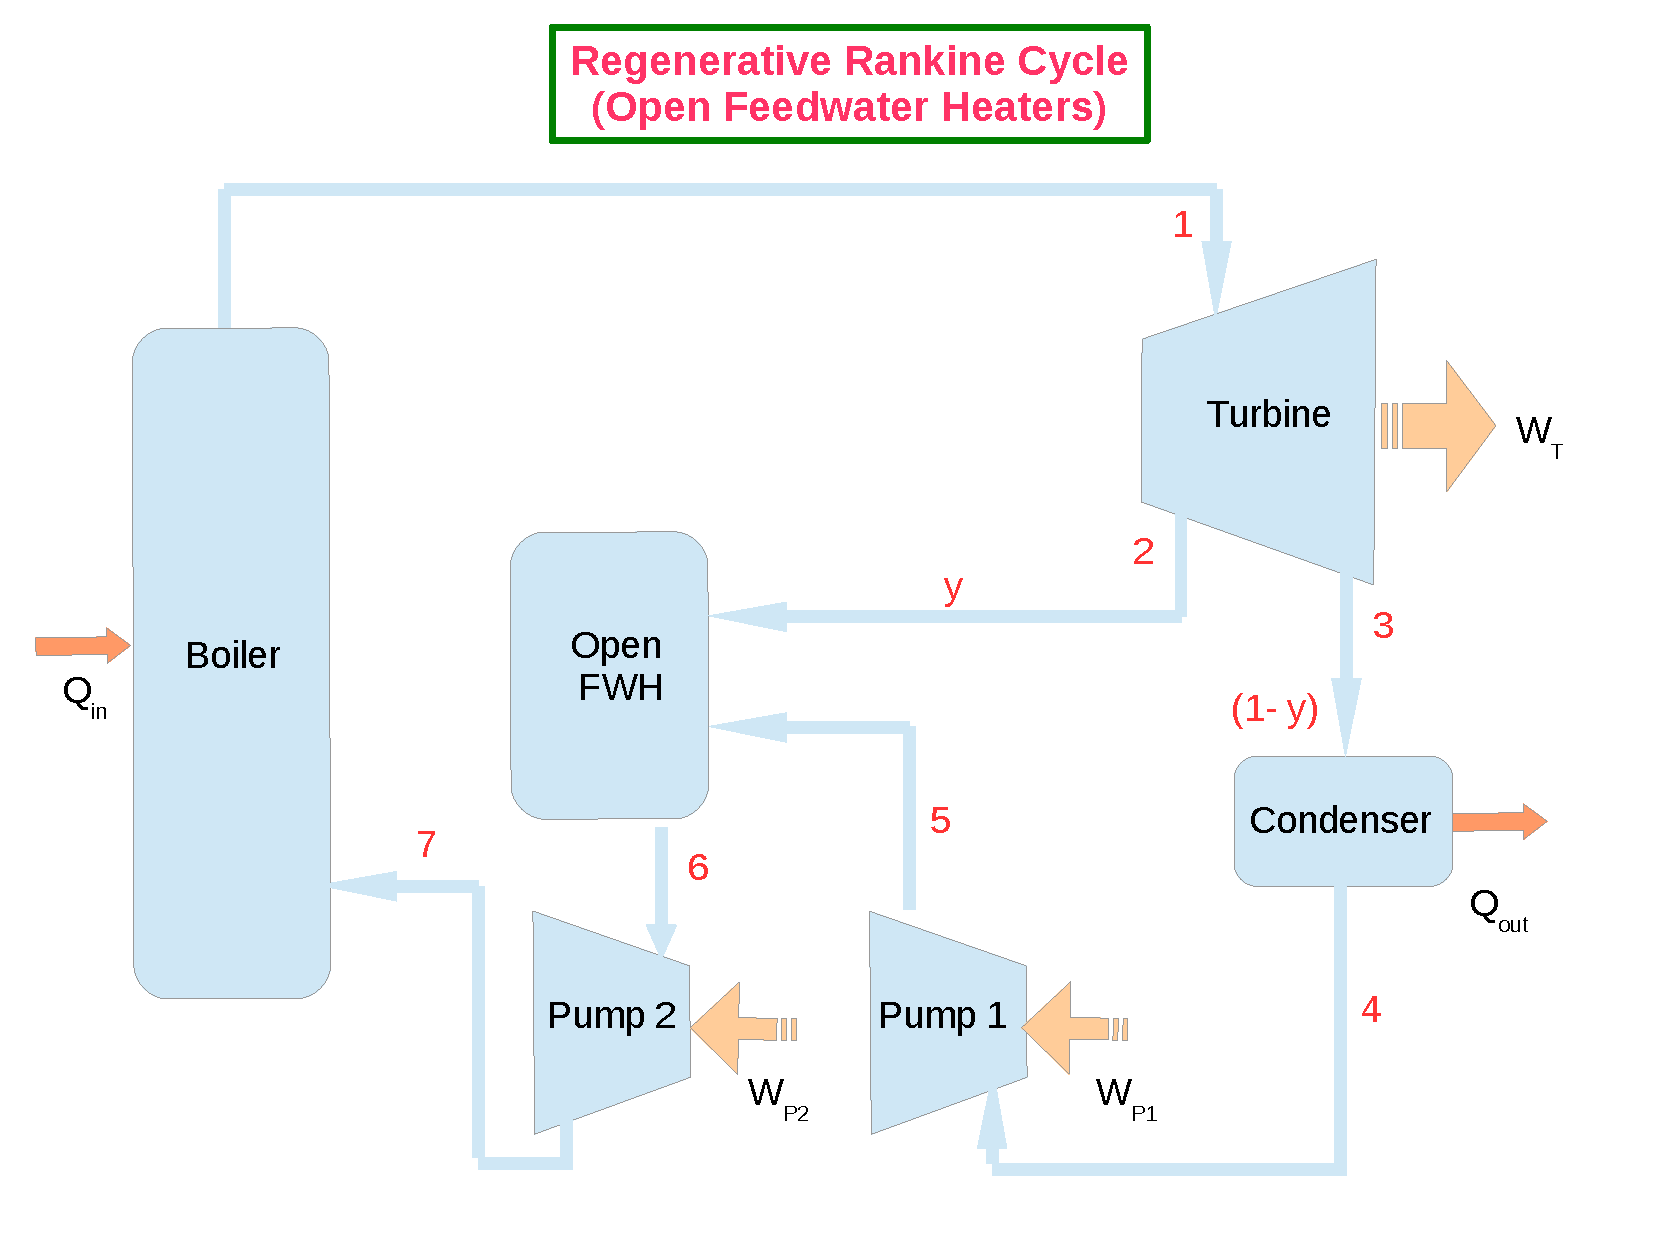
\includegraphics[width=6.cm,clip]{./Pics/RegenerativeOpen_RankineCycle}}
%         \vspace{-0.7cm}
%         \hbox{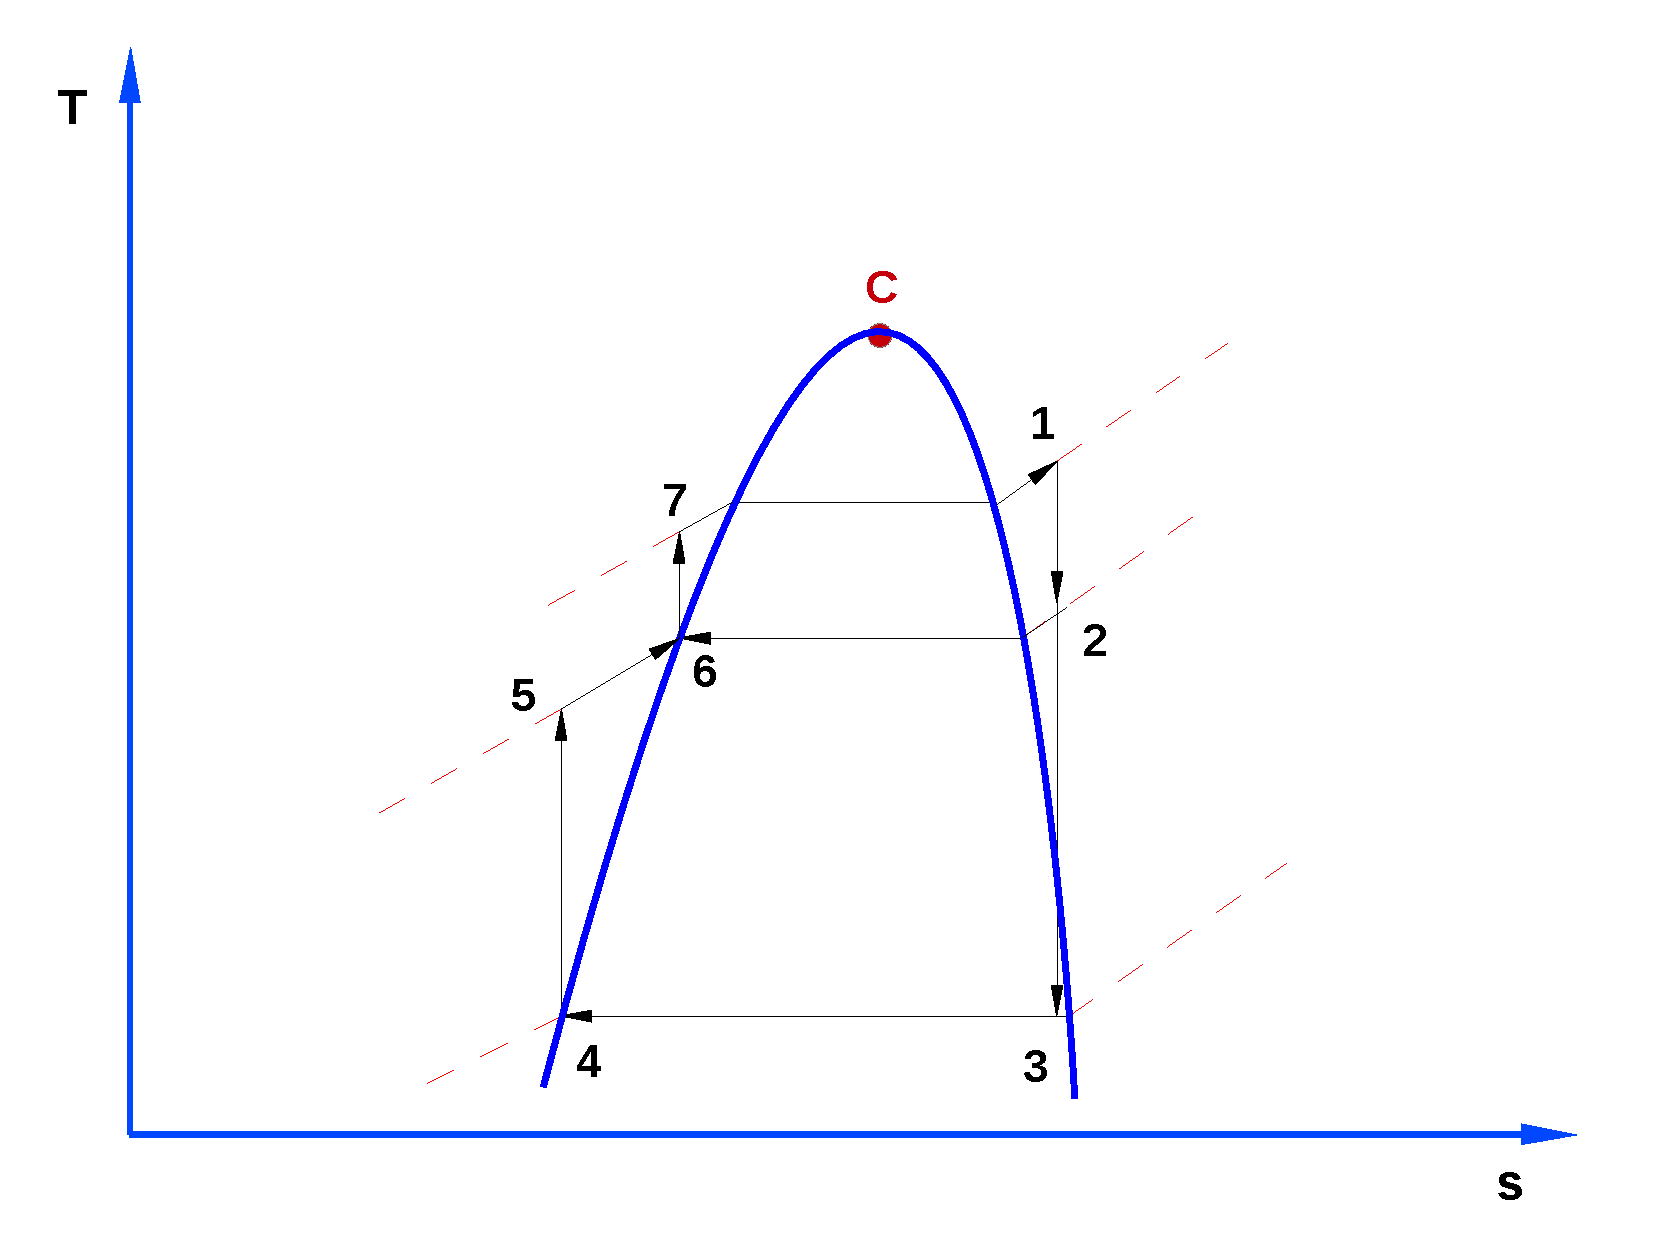
\includegraphics[width=6.cm,clip]{./Pics/RegenerativeOpen_RankineCycle_Diagram}}
%      }  
